\documentclass{beamer}
\usepackage[utf8]{inputenc}
\usepackage[T1]{fontenc}
\usepackage[english]{babel}
\usepackage{lmodern}
\usepackage{amsmath}
\usepackage{amssymb}
\usepackage{amsthm}
\usepackage[superscript]{cite}
\usepackage{nicefrac}
\usepackage{upgreek}
\usepackage{paralist}
\usepackage{stmaryrd}
\usepackage{tikz}
\usepackage{graphicx}
\usepackage{qtree}
\usepackage{dsfont}
\usepackage{eurosym}
\usepackage{tabulary}
\usepackage{setspace}
% \usepackage[colorlinks=true,linkcolor=blue]{hyperref}				% Blaue Links sehen meiner Ansicht nach besser aus als die rot umrandeten Verweise

\usetheme{Madrid}				% Verwende Goettingen für TOC auf jeder Seite, Madrid ohne Navigation

% Kommandos, Operatoren, etc.
\newcommand{\abs}[1]{\lvert#1\rvert}
\newcommand{\norm}[1]{\lVert#1\rVert}
\DeclareMathOperator{\thetafunc}{\uptheta}

% ENDE PRÄAMBEL

\author{Dominik Blank}
\title{Gleichmäßige obere Schranken beim Kreisproblem}

\setlength{\parindent}{0pt}
\allowdisplaybreaks

\begin{document}

\begin{frame}
	\tableofcontents
\end{frame}

\begin{frame}
	\section{ROI Testing}
	
	\subsection{The statistical model}
	
	Let $M, N \in \mathbb{N}$ and $G = \left\{ 0, \dots, M-1 \right\} \times  \left\{ 0, \dots, N-1 \right\}$. Assume we are given data
	\begin{equation}\label{f}
		f(m, n) = c_{bg} + v(m, n) + \varepsilon_{m, n}
	\end{equation}
	where $(m, n) \in G$, $c_{bg} \in \mathbb{R}$ is constant, $v: G \to \{ 0, \pm c_{bg} \}$ and $\varepsilon_{m, n} \sim \mathcal{N}(0, \sigma^2)$ are i.i.d. normal distributed random variables for some $\sigma > 0$ and for all $(m, n) \in G$.
	
	We treat $v$ as an image, that contains a rectangular, thus convex, region of interest. That means, that the pixels with value $\pm c_{bg}$ are arranged in a rectangular shape and all other pixels have value $0$.
\end{frame}

\begin{frame}
	\subsection{Testing for the ROI}
	
	\subsubsection{Preparations}
	
	For each pair $(m, n) \in G$ we define four values
	\begin{align}
		\tilde{d}^\pm_1(m, n) &= f(m \pm 1, n) - f(m, n) \label{d1} \\
		\tilde{d}^\pm_2(m, n) &= f(m, n \pm 1) - f(m, n) \label{d2}
	\end{align}
	We now combine these values into two new values and assign to each pair $(m, n) \in G$ the values
	\begin{equation}\label{d_tilde}
		\tilde{d}^\pm(m, n) = \sqrt{\tilde{d}_1^\pm(m, n)^2 + \tilde{d}_2^\pm(m, n)^2}
	\end{equation}
\end{frame}

\begin{frame}
	We now want to test if a pixel is part of the aforementioned region of interest (ROI). To do this, we define another two values for each pixel $(m, n) \in G$:
	\begin{equation}\label{d}
		d^\pm(m, n) = \sqrt{(v(m \pm 1, n) - v(m, n))^2 + (v(m, n \pm 1) - v(m, n))^2}
	\end{equation}
	The definition of $d^\pm(m, n)$ helps us define a null hypothesis for our testing procedure. If a pixel is background and since we assumed the ROI to be rectangular, that means, that its top and left neighbour pixels or bottom and right neighbour pixels are background as well. This leads to the null hypothesis
	\begin{equation}
		H_0 : \min\{ d^+(m, n), d^-(m, n) \} = 0
	\end{equation}
	Since by definition $d^\pm(m, n) \geq 0$, our alternative hypothesis becomes
	\begin{equation}
		H_1 : \min\{ d^+(m, n), d^-(m, n) \} > 0
	\end{equation}
\end{frame}

\begin{frame}
	Since $v$ only takes values in $\{ 0, -c_{bg}, c_{bg} \}$, $d^\pm$ also can only attain values in
	\begin{equation*}
		\mathcal{D} = \{ 0, c_{bg}, 2 c_{bg}, \sqrt{2} c_{bg}, \sqrt{5} c_{bg}, \sqrt{8} c_{bg} \}
	\end{equation*}
	This means, that we can define two sets $\mathcal{D}_0$ and $\mathcal{D}_1$ as follows
	\begin{equation*}
		\mathcal{D}_1 = ( \mathcal{D} \setminus \{ 0 \} ) \times ( \mathcal{D} \setminus \{ 0 \} )
	\end{equation*}
	\begin{equation*}
		\mathcal{D}_0 = ( \mathcal{D} \setminus \{ 0 \} ) \times \{ 0 \} \cup \{ 0 \} \times ( \mathcal{D} \setminus \{ 0 \} ) \cup ( \{ 0 \} \times \{ 0 \} ) = ( \mathcal{D} \times \mathcal{D} ) \setminus \mathcal{D}_1
	\end{equation*}
	Now, if $(d^+, d^-) \in \mathcal{D}_0$ then the null hypothesis is true and if $(d^+, d^-) \in \mathcal{D}_1$, the alternative hypothesis is true.
\end{frame}

\begin{frame}
	\subsubsection{Distribution of $\mathbb{P}(\tilde{d}^\pm(m, n) \leq t \mid d^\pm(m, n) = d)$}
	
	We want to determine the distribution of $\tilde{d}^\pm(m, n)$ conditioned on $d^\pm(m, n) = d$ for some $d \in \mathcal{D}$. We define
	\begin{align*}
		d_1^\pm(m, n) &= v(m \pm 1, n) - v(m, n) \\
		d_2^\pm(m, n) &= v(m, n \pm 1) - v(m, n)
	\end{align*}
	Then $d^\pm(m, n) = \sqrt{d_1^\pm(m, n)^2 + d_2^\pm(m, n)^2}$. We note that the roles of $d_1^\pm(m, n)$ and $d_2^\pm(m, n)$ are symmetrical. Furthermore we can see, that for $d^\pm(m, n) = d$ given, we can determine, what $d_1^\pm(m, n)$ and $d_2^\pm(m, n)$ are.
\end{frame}

\begin{frame}
	\begin{center}
		\begin{tabular}{c|c|c}
			$d$ & $d_1^\pm$ & $d_2^\pm$ \\
			\hline
			$0$ & $0$ & $0$ \\
			\hline
			$c_{bg}$ & $\{ c_{bg}, 0 \}$ & $\{ 0, c_{bg} \}$ \\
			\hline
			$2 c_{bg}$ & $\{ 2 c_{bg}, 0 \}$ & $\{ 0, 2 c_{bg} \}$ \\
			\hline
			$\sqrt{2} c_{bg}$ & $c_{bg}$ & $c_{bg}$ \\
			\hline
			$\sqrt{5} c_{bg}$ & $\{ 2 c_{bg}, c_{bg} \}$ & $\{ c_{bg}, 2 c_{bg} \}$ \\
			\hline
			$\sqrt{8} c_{bg}$ & $2 c_{bg}$ & $2 c_{bg}$ \\
		\end{tabular}
	\end{center}
\end{frame}

\begin{frame}
	Using this relation, we get
	\begin{equation*}
		\mathbb{P}(\tilde{d}^\pm(m, n) \leq t \mid d^\pm(m, n) = d) = \mathbb{P}\left( \sqrt{2} \sigma \sqrt{\left( \frac{X_1}{\sqrt{2} \sigma} \right)^2 + \left( \frac{X_2}{\sqrt{2} \sigma} \right)^2} \leq t \right)
	\end{equation*}
	with
	\begin{align*}
		X_1 &= d_1^\pm(m, n) + \varepsilon_{m \pm 1, n} - \varepsilon_{m, n} \sim \mathcal{N}(d_1^\pm(m, n), 2 \sigma^2) \\
		X_2 &= d_2^\pm(m, n) + \varepsilon_{m, n \pm 1} - \varepsilon_{m, n} \sim \mathcal{N}(d_2^\pm(m, n), 2 \sigma^2)
	\end{align*}
	
	Then we can see, that the square root inside has non-central chi distribution with two degrees of freedom and parameter
	\begin{equation*}
		\lambda = \sqrt{\left( \frac{d_1^\pm}{\sqrt{2} \sigma} \right)^2 + \left( \frac{d_2^\pm}{\sqrt{2} \sigma} \right)^2} = \frac{\sqrt{d_1^\pm(m, n)^2 + d_2^\pm(m, n)^2}}{\sqrt{2} \sigma} = \frac{d^\pm(m, n)}{\sqrt{2} \sigma}
	\end{equation*}
\end{frame}

\begin{frame}
	The cumulative distribution function of the non-central chi distribution with parameter $\lambda$ and two degrees of freedom is $1 - Q_1(\lambda, x)$, where $Q_M(a, b)$ denotes the Marcum $Q$-function, which is defined as
	\begin{equation*}
		Q_M(a, b) = \int_b^\infty x \left( \frac{x}{a} \right)^{M-1} \exp \left( - \frac{x^2 + a^2}{2} \right) I_{M-1}(ax) dx
	\end{equation*}
	with modified Bessel function $I_{M-1}$.
	
	Putting this together, we obtain
	\begin{align*}
		\mathbb{P}(\tilde{d}^\pm(m, n) \leq t \mid d^\pm(m, n) = d) &= \mathbb{P}\left( \sqrt{\left( \frac{X_1}{\sqrt{2} \sigma} \right)^2 + \left( \frac{X_2}{\sqrt{2} \sigma} \right)^2} \leq \frac{t}{\sqrt{2} \sigma} \right) \\
		&= 1 - Q_1 \left( \frac{d}{\sqrt{2} \sigma}, \frac{t}{\sqrt{2} \sigma} \right)
	\end{align*}
	
	For $d = 0$ this simplifies a lot and we get
	\begin{equation*}
		\mathbb{P}(\tilde{d}^\pm(m, n) \leq t \mid d^\pm(m, n) = 0) = 1 - \exp \left( - \frac{t^2}{4 \sigma^2} \right)
	\end{equation*}
\end{frame}

\begin{frame}
	\subsubsection{Statistical significance}
	We use $T = \tilde{d}(m, n) = \min \{ \tilde{d}^+(m, n), \tilde{d}^-(m, n) \}$ as our test statistic. Dropping $(m, n)$ in every term for readability, we get
	\begin{equation*}
		\mathbb{P}(T \geq t \mid H_0) \leq \exp \left( - \frac{t^2}{4 \sigma^2} \right)
	\end{equation*}
\end{frame}

\begin{frame}
	\subsubsection{Power of the test}
	After having established an upper bound for the statistical significance, we aim to provide a lower and upper bound for the power of our test. Especially the upper bound will be quite loose.
	
	Using results and notations from the previous sections, we get the lower bound
	\begin{equation*}
		\beta = \mathbb{P}(T \leq t \mid H_1) \geq 1 - Q_1 \left( \frac{2 c_{bg}}{\sigma}, \frac{t}{\sqrt{2} \sigma} \right)
	\end{equation*}
	
	On the other hand, we get the upper bound
	\begin{equation*}
		\beta = \mathbb{P}(T \leq t \mid H_1) \leq 2 \cdot \left( 1 - Q_1 \left( \frac{c_{bg}}{\sqrt{2} \sigma}, \frac{t}{\sqrt{2} \sigma} \right) \right)
	\end{equation*}
	
	Thus we can conclude, that
	\begin{equation*}
		\beta \in \left[ 1 - Q_1 \left( \frac{2 c_{bg}}{\sigma}, \frac{t}{\sqrt{2} \sigma} \right), \min \left\{ 2 \cdot \left( 1 - Q_1 \left( \frac{c_{bg}}{\sqrt{2} \sigma}, \frac{t}{\sqrt{2} \sigma} \right) \right), 1 \right\} \right]
	\end{equation*}
\end{frame}

\begin{frame}
	\subsubsection{Numerical results}
	
	In the case of a grayscale image, we assume $c_{bg} = 127.5$. As we have seen $\mathbb{P}(T \geq t \mid H_0) \leq \exp \left( - \frac{t^2}{4 \sigma^2} \right)$. By taking $t = 2 \sigma \sqrt{- \log(\alpha)}$ we thus can assure a statistical significance of $\alpha$.
	
	\begin{figure}[h]
		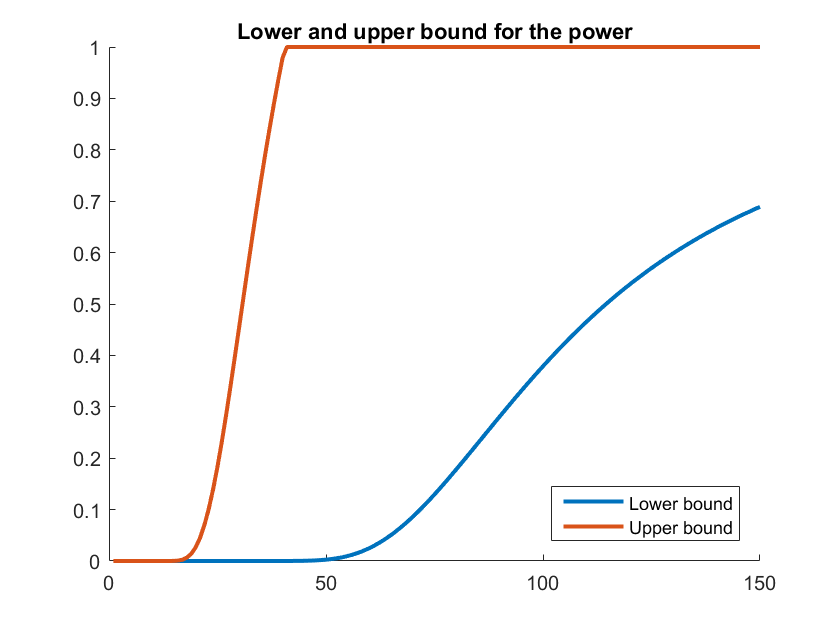
\includegraphics[width=0.6\linewidth]{Power_Bounds}
		\caption[Power bounds]{For $\alpha = 0.05$ this graph shows the lower and upper bounds for the power of the test for $\sigma \in \{ 1, 2, \dots, 150 \}$.}
		\label{fig:demo1comparison}
	\end{figure}
\end{frame}

\begin{frame}
	As we can see in the graph, we can assure, that there are no type II errors for $\sigma \in \{ 1, 2, \dots, 8 \}$. Up until $\sigma = 21$ the power stays below $\alpha = 0.05$. The upper bound increases then very fast and starting at $\sigma = 41$ we can only use the trivial upper bound, i.e. $1$. The lower bound stays at $0$ until $\sigma = 23$ and increases slowly. At $\sigma = 115$ it becomes bigger than $0.5$.
\end{frame}

\begin{frame}
	\section{Morphological operations}
	
	\subsection{Opening and closing}
	
	To define opening and closing, we first need to define erosion and dilation of binary images.
	
	\begin{definition}
		Let $A, B \subseteq \mathbb{R}^m$. The binary erosion of $A$ by $B$ is defined as
		\begin{equation*}
			A \ominus_b B = \left\{ x \in \mathbb{R}^m \mid x + b \in A \; \mathrm{for \; every} \; b \in B \right\}
		\end{equation*}
	\end{definition}
	\begin{definition}
		Let $A, B \subseteq \mathbb{R}^m$. The binary dilation of $A$ by $B$ is defined as
		\begin{equation*}
			A \oplus_b B = \left\{ c \in \mathbb{R}^m \mid c = a + b \; \mathrm{for \; some} \; a \in A \; \mathrm{and} \; b \in B \right\}
		\end{equation*}
	\end{definition}
	
	This can be rewritten in a more implementation-friendly form:
	\begin{align*}
		(A \ominus_b B)_{(i, j)} &= \underset{m, n}{\mathrm{AND}} \left( \mathrm{OR} (A_{(i + m, j + n)}, (1 - B)_{(m, n)}) \right) \\
		(A \oplus_b B)_{(i, j)} &= \underset{m, n}{\mathrm{OR}} \left( \mathrm{AND} (A_{(i - m, j - n)}, B_{(m, n)}) \right)
	\end{align*}
	Where $m, n$ go through the indices, where $B = 1$.
\end{frame}

\begin{frame}
	Now we can define binary opening and closing.
	
	\begin{definition}
		The opening of an image $A$ by a structuring element $B$ is defined as
		\begin{equation*}
			A \circ B = (A \ominus B) \oplus B
		\end{equation*}
	\end{definition}
	\begin{definition}
		The closing of an image $A$ by a structuring element $B$ is defined as
		\begin{equation*}
			A \bullet B = (A \oplus B) \ominus B
		\end{equation*}
	\end{definition}
\end{frame}

\begin{frame}
	\subsection{Hypothesis testing and opening}
	
	From now on, we assume $B$ to be a square of ones centered around our current pixel. Using the notation from above we can take a closer look at what opening really does. We have
	\begin{equation*}
		(A \circ B)_{(i, j)} = ((A \ominus B) \oplus B)_{(i, j)} = \underset{\tilde{m}, \tilde{n}}{\mathrm{OR}} \left( \underset{m, n}{\mathrm{AND}} ( A_{(i + m - \tilde{m}, j + n - \tilde{n})} ) \right)
	\end{equation*}
	
	Now, we can see, that $A \circ B_{(i, j)} = 1$ if and only if $(i, j)$ is part of a square the size of $B$. In the above formula $(\tilde{m}, \tilde{n})$ determines the offset of the center of the square and thus loops through all possible positions of $(i, j)$ in the square. The inner part on the other hand assures, that there is actually a square of same size as $B$, that $(i, j)$ is part of.
\end{frame}

\begin{frame}
	We will now take a look at the effect of opening on the significance level.
	
	\begin{theorem}
		Let $f$ be an image that contains a rectangular ROI. Assume that we are given a binarized image $f_{bin}$ with
		\begin{equation*}
			\mathbb{P}(f_{bin}(i, j) = 1 \mid H_0(i, j)) \leq \alpha
		\end{equation*}
		where $H_0(i, j)$ denotes the null hypothesis for the pixel $(i, j)$, which is, that it is a background pixel and thus should be set to zero.
		
		Let $k \in \mathbb{N}$ be odd and $B$ be a square structuring element with side length $k$. For $\tilde{m}, \tilde{n} \in \{ -\frac{k - 1}{2}, \dots, \frac{k - 1}{2} \}$ we denote by $\mathcal{G}_{(\tilde{m}, \tilde{n})}^k(i, j)$ the set of all possible ground truths in the square with side length $k$, where the pixel $(i, j)$ has offest $(\tilde{m}, \tilde{n})$ from the center of the square and assuming that the null hypothesis for the pixel $(i, j)$ is true.
		Then the following inequality holds:
		\begin{equation*}
			\mathbb{P}((f_{bin} \circ B)(i, j) = 1 \mid H_0(i, j)) \leq k^2 \alpha^k
		\end{equation*}
	\end{theorem}
\end{frame}

\begin{frame}
	\subsection{Hypothesis testing and closing}
	In a similar way as above, we can also see, what closing does. We have
	\begin{equation*}
		(A \bullet B)_{(i, j)} = ((A \oplus B) \ominus B)_{(i, j)} = \underset{\tilde{m}, \tilde{n}}{\mathrm{AND}} \left( \underset{m, n}{\mathrm{OR}} ( A_{(i - m + \tilde{m}, j - n + \tilde{n})} ) \right)
	\end{equation*}
\end{frame}

\begin{frame}
	\subsection{Convex hull}
	
	As we have seen in the section about multiple testing procedures, we defined the family-wise error rate as $\mathbb{P}(V \geq 1) = 1 - \mathbb{P}(V = 0)$.
\end{frame}

\begin{frame}
	\section{Multiple testing procedures}
	
	Consider the following setup:
	\begin{table}[h]
		\tymax .3\textwidth
		\begin{tabulary}{\textwidth}{|CCCC|}
			\hline
			& \textit{Declared non-significant} & \textit{Declared significant} & \textit{Total} \\
			\hline
			\textit{True null hypotheses} & $\mathbf{U}$ & $\mathbf{V}$ & $m_0$ \\
			\textit{Non-true null hypotheses} & $\mathbf{T}$ & $\mathbf{S}$ & $m - m_0$ \\
			& $m - \mathbf{R}$ & $\mathbf{R}$ & $m$ \\
			\hline
		\end{tabulary}
	\end{table}
\end{frame}

\begin{frame}
	\begin{itemize}
		\item $m$ is the total number hypotheses tested
		\item $m_0$ is the number of true null hypotheses, an unknown parameter
		\item $m - m_0$ is the number of true alternative hypotheses
		\item $V$ is the number of false positives (Type I error) (also called "false discoveries")
		\item $S$ is the number of true positives
		\item $T$ is the number of false negatives (Type II error)
		\item $U$ is the number of true negatives
		\item $R = V + S$ is the number of rejected null hypotheses (also called "discoveries", either true or false)
	\end{itemize}
	In $m$ hypothesis tests of which $m_0$ are true null hypotheses, $R$ is an observable random variable, and $S$, $T$, $U$, and $V$ are unobservable random variables.
\end{frame}

\begin{frame}
	We define another random variable $Q = \frac{V}{V + S}$, which is the proportion of the rejected null hypotheses which are erroneously rejected. We set $Q = 0$, if $V + S = 0$. Based on this, we define the false discovery rate to be
	\begin{equation}
		FDR = \mathbb{E}(Q) = \mathbb{E} \left( \frac{V}{V + S} \right)
	\end{equation}
	
	We also define the family-wise error rate to be
	\begin{equation}
		FWER = \mathbb{P}( V \geq 1 ) = 1 - \mathbb{P}( V = 0 )
	\end{equation}
	that is the probability of making one or more type I errors.
\end{frame}

\begin{frame}
	Three of these multiple testing procedures are given in detail in the following. The first one controls the false discovery rate at level $\alpha$, i.e.
	\begin{equation}
		FDR = \mathbb{E}(Q) \leq \alpha
	\end{equation}
	
	The other two procedures control the family-wise error rate at level $\alpha$, i.e.
	\begin{equation}
		FWER = \mathbb{P}( V \geq 1 ) \leq \alpha
	\end{equation}
\end{frame}

\begin{frame}
	First, we calculate for every pixel $(m, n) \in G$ the $p$-value
	\begin{equation}
		p(m, n) = \exp \left( - \frac{\tilde{d}(m, n)^2}{4 \sigma^2} \right) \geq \mathbb{P}(T \geq \tilde{d}(m, n) \mid H_0)
	\end{equation}
\end{frame}

\begin{frame}
	\subsection{FDR Thresholding}
	
	\begin{itemize}
		\item Sort $p$-values in ascending order: $p_{(1)} \leq p_{(2)} \leq \dots \leq p_{(M \cdot N)}$
		\item Calculate the maximal index $k$, such that $p_{(k)} \leq \frac{k \cdot \alpha}{M \cdot N}$
		\item Calculate the threshold $\lambda_{k} = 2 \sigma \sqrt{- \log(p_{(k)})}$
		\item Reject all hypotheses $H_{(i)}$ with $p_{(i)} \leq p_{(k)}$, i.e. all hypotheses with $$\tilde{d}_{(i)} \geq \tilde{d}_{(k)} = \lambda_{k} = 2 \sigma \sqrt{- \log(p_{(k)})}$$
	\end{itemize}
\end{frame}

\begin{frame}
	\subsection{Bonferroni Thresholding}
	
	\begin{itemize}
		\item Reject all hypotheses $H_{i}$ with $p_{i} \leq \frac{\alpha}{M \cdot N}$, i.e. all hypotheses with $$\tilde{d}_{i} \geq \lambda_k = 2 \sigma \sqrt{- \log \left( \frac{\alpha}{M \cdot N} \right)}$$
	\end{itemize}
\end{frame}

\begin{frame}
	\subsection{Hochberg Thresholding}
	
	\begin{itemize}
		\item Sort $p$-values in ascending order: $p_{(1)} \leq p_{(2)} \leq \dots \leq p_{(M \cdot N)}$
		\item Calculate the maximal index $k$, such that $p_{(k)} \leq \frac{\alpha}{M \cdot N - k + 1}$
		\item Reject all hypotheses $H_{(i)}$ with $p_{(i)} \leq p_{(k)}$, i.e. all hypotheses with $$\tilde{d}_{(i)} \geq \tilde{d}_{(k)} = \lambda_{k} = 2 \sigma \sqrt{- \log(p_{(k)})}$$
	\end{itemize}
\end{frame}

\begin{frame}
	All these methods are defined for actual $p$-values, i.e.
	\begin{equation*}
		p(m, n) = \mathbb{P}(T \geq \tilde{d}(m, n) \mid H_0)
	\end{equation*}
	In contrast to that, we have taken upper bounds for the $p$-values. This is not an issue though, since by taking upper bounds we might decrease the number of hypotheses we reject. Thus it will not increase the error rate.
	
	The threshold has the following interpretation:
	\begin{itemize}
		\item If $\tilde{d}(m, n) \geq \lambda_{k}$, then $(m, n)$ is part of the ROI.
		\item If $\tilde{d}(m, n) < \lambda_{k}$, then $(m, n)$ is NOT part of the ROI.
	\end{itemize}
\end{frame}


\end{document}
